\documentclass{article} % For LaTeX2e
\usepackage{icomp2026_conference,times}
\usepackage{amsmath}
\usepackage{amssymb}
\usepackage{amsfonts}
\usepackage{graphicx}
\usepackage{booktabs}
\usepackage{bbold}
\usepackage{amsthm}
\usepackage{float}
\usepackage{placeins}
% Optional math command from https://github.com/goodfeli/dlbook_notation.
%%%%% NEW MATH DEFINITIONS %%%%%

\usepackage{amsmath,amsfonts,bm}

% Mark sections of captions for referring to divisions of figures
\newcommand{\figleft}{{\em (Left)}}
\newcommand{\figcenter}{{\em (Center)}}
\newcommand{\figright}{{\em (Right)}}
\newcommand{\figtop}{{\em (Top)}}
\newcommand{\figbottom}{{\em (Bottom)}}
\newcommand{\captiona}{{\em (a)}}
\newcommand{\captionb}{{\em (b)}}
\newcommand{\captionc}{{\em (c)}}
\newcommand{\captiond}{{\em (d)}}

% Highlight a newly defined term
\newcommand{\newterm}[1]{{\bf #1}}


% Figure reference, lower-case.
\def\figref#1{figure~\ref{#1}}
% Figure reference, capital. For start of sentence
\def\Figref#1{Figure~\ref{#1}}
\def\twofigref#1#2{figures \ref{#1} and \ref{#2}}
\def\quadfigref#1#2#3#4{figures \ref{#1}, \ref{#2}, \ref{#3} and \ref{#4}}
% Section reference, lower-case.
\def\secref#1{section~\ref{#1}}
% Section reference, capital.
\def\Secref#1{Section~\ref{#1}}
% Reference to two sections.
\def\twosecrefs#1#2{sections \ref{#1} and \ref{#2}}
% Reference to three sections.
\def\secrefs#1#2#3{sections \ref{#1}, \ref{#2} and \ref{#3}}
% Reference to an equation, lower-case.
\def\eqref#1{equation~\ref{#1}}
% Reference to an equation, upper case
\def\Eqref#1{Equation~\ref{#1}}
% A raw reference to an equation---avoid using if possible
\def\plaineqref#1{\ref{#1}}
% Reference to a chapter, lower-case.
\def\chapref#1{chapter~\ref{#1}}
% Reference to an equation, upper case.
\def\Chapref#1{Chapter~\ref{#1}}
% Reference to a range of chapters
\def\rangechapref#1#2{chapters\ref{#1}--\ref{#2}}
% Reference to an algorithm, lower-case.
\def\algref#1{algorithm~\ref{#1}}
% Reference to an algorithm, upper case.
\def\Algref#1{Algorithm~\ref{#1}}
\def\twoalgref#1#2{algorithms \ref{#1} and \ref{#2}}
\def\Twoalgref#1#2{Algorithms \ref{#1} and \ref{#2}}
% Reference to a part, lower case
\def\partref#1{part~\ref{#1}}
% Reference to a part, upper case
\def\Partref#1{Part~\ref{#1}}
\def\twopartref#1#2{parts \ref{#1} and \ref{#2}}

\def\ceil#1{\lceil #1 \rceil}
\def\floor#1{\lfloor #1 \rfloor}
\def\1{\bm{1}}
\newcommand{\train}{\mathcal{D}}
\newcommand{\valid}{\mathcal{D_{\mathrm{valid}}}}
\newcommand{\test}{\mathcal{D_{\mathrm{test}}}}

\def\eps{{\epsilon}}


% Random variables
\def\reta{{\textnormal{$\eta$}}}
\def\ra{{\textnormal{a}}}
\def\rb{{\textnormal{b}}}
\def\rc{{\textnormal{c}}}
\def\rd{{\textnormal{d}}}
\def\re{{\textnormal{e}}}
\def\rf{{\textnormal{f}}}
\def\rg{{\textnormal{g}}}
\def\rh{{\textnormal{h}}}
\def\ri{{\textnormal{i}}}
\def\rj{{\textnormal{j}}}
\def\rk{{\textnormal{k}}}
\def\rl{{\textnormal{l}}}
% rm is already a command, just don't name any random variables m
\def\rn{{\textnormal{n}}}
\def\ro{{\textnormal{o}}}
\def\rp{{\textnormal{p}}}
\def\rq{{\textnormal{q}}}
\def\rr{{\textnormal{r}}}
\def\rs{{\textnormal{s}}}
\def\rt{{\textnormal{t}}}
\def\ru{{\textnormal{u}}}
\def\rv{{\textnormal{v}}}
\def\rw{{\textnormal{w}}}
\def\rx{{\textnormal{x}}}
\def\ry{{\textnormal{y}}}
\def\rz{{\textnormal{z}}}

% Random vectors
\def\rvepsilon{{\mathbf{\epsilon}}}
\def\rvtheta{{\mathbf{\theta}}}
\def\rva{{\mathbf{a}}}
\def\rvb{{\mathbf{b}}}
\def\rvc{{\mathbf{c}}}
\def\rvd{{\mathbf{d}}}
\def\rve{{\mathbf{e}}}
\def\rvf{{\mathbf{f}}}
\def\rvg{{\mathbf{g}}}
\def\rvh{{\mathbf{h}}}
\def\rvu{{\mathbf{i}}}
\def\rvj{{\mathbf{j}}}
\def\rvk{{\mathbf{k}}}
\def\rvl{{\mathbf{l}}}
\def\rvm{{\mathbf{m}}}
\def\rvn{{\mathbf{n}}}
\def\rvo{{\mathbf{o}}}
\def\rvp{{\mathbf{p}}}
\def\rvq{{\mathbf{q}}}
\def\rvr{{\mathbf{r}}}
\def\rvs{{\mathbf{s}}}
\def\rvt{{\mathbf{t}}}
\def\rvu{{\mathbf{u}}}
\def\rvv{{\mathbf{v}}}
\def\rvw{{\mathbf{w}}}
\def\rvx{{\mathbf{x}}}
\def\rvy{{\mathbf{y}}}
\def\rvz{{\mathbf{z}}}

% Elements of random vectors
\def\erva{{\textnormal{a}}}
\def\ervb{{\textnormal{b}}}
\def\ervc{{\textnormal{c}}}
\def\ervd{{\textnormal{d}}}
\def\erve{{\textnormal{e}}}
\def\ervf{{\textnormal{f}}}
\def\ervg{{\textnormal{g}}}
\def\ervh{{\textnormal{h}}}
\def\ervi{{\textnormal{i}}}
\def\ervj{{\textnormal{j}}}
\def\ervk{{\textnormal{k}}}
\def\ervl{{\textnormal{l}}}
\def\ervm{{\textnormal{m}}}
\def\ervn{{\textnormal{n}}}
\def\ervo{{\textnormal{o}}}
\def\ervp{{\textnormal{p}}}
\def\ervq{{\textnormal{q}}}
\def\ervr{{\textnormal{r}}}
\def\ervs{{\textnormal{s}}}
\def\ervt{{\textnormal{t}}}
\def\ervu{{\textnormal{u}}}
\def\ervv{{\textnormal{v}}}
\def\ervw{{\textnormal{w}}}
\def\ervx{{\textnormal{x}}}
\def\ervy{{\textnormal{y}}}
\def\ervz{{\textnormal{z}}}

% Random matrices
\def\rmA{{\mathbf{A}}}
\def\rmB{{\mathbf{B}}}
\def\rmC{{\mathbf{C}}}
\def\rmD{{\mathbf{D}}}
\def\rmE{{\mathbf{E}}}
\def\rmF{{\mathbf{F}}}
\def\rmG{{\mathbf{G}}}
\def\rmH{{\mathbf{H}}}
\def\rmI{{\mathbf{I}}}
\def\rmJ{{\mathbf{J}}}
\def\rmK{{\mathbf{K}}}
\def\rmL{{\mathbf{L}}}
\def\rmM{{\mathbf{M}}}
\def\rmN{{\mathbf{N}}}
\def\rmO{{\mathbf{O}}}
\def\rmP{{\mathbf{P}}}
\def\rmQ{{\mathbf{Q}}}
\def\rmR{{\mathbf{R}}}
\def\rmS{{\mathbf{S}}}
\def\rmT{{\mathbf{T}}}
\def\rmU{{\mathbf{U}}}
\def\rmV{{\mathbf{V}}}
\def\rmW{{\mathbf{W}}}
\def\rmX{{\mathbf{X}}}
\def\rmY{{\mathbf{Y}}}
\def\rmZ{{\mathbf{Z}}}

% Elements of random matrices
\def\ermA{{\textnormal{A}}}
\def\ermB{{\textnormal{B}}}
\def\ermC{{\textnormal{C}}}
\def\ermD{{\textnormal{D}}}
\def\ermE{{\textnormal{E}}}
\def\ermF{{\textnormal{F}}}
\def\ermG{{\textnormal{G}}}
\def\ermH{{\textnormal{H}}}
\def\ermI{{\textnormal{I}}}
\def\ermJ{{\textnormal{J}}}
\def\ermK{{\textnormal{K}}}
\def\ermL{{\textnormal{L}}}
\def\ermM{{\textnormal{M}}}
\def\ermN{{\textnormal{N}}}
\def\ermO{{\textnormal{O}}}
\def\ermP{{\textnormal{P}}}
\def\ermQ{{\textnormal{Q}}}
\def\ermR{{\textnormal{R}}}
\def\ermS{{\textnormal{S}}}
\def\ermT{{\textnormal{T}}}
\def\ermU{{\textnormal{U}}}
\def\ermV{{\textnormal{V}}}
\def\ermW{{\textnormal{W}}}
\def\ermX{{\textnormal{X}}}
\def\ermY{{\textnormal{Y}}}
\def\ermZ{{\textnormal{Z}}}

% Vectors
\def\vzero{{\bm{0}}}
\def\vone{{\bm{1}}}
\def\vmu{{\bm{\mu}}}
\def\vtheta{{\bm{\theta}}}
\def\va{{\bm{a}}}
\def\vb{{\bm{b}}}
\def\vc{{\bm{c}}}
\def\vd{{\bm{d}}}
\def\ve{{\bm{e}}}
\def\vf{{\bm{f}}}
\def\vg{{\bm{g}}}
\def\vh{{\bm{h}}}
\def\vi{{\bm{i}}}
\def\vj{{\bm{j}}}
\def\vk{{\bm{k}}}
\def\vl{{\bm{l}}}
\def\vm{{\bm{m}}}
\def\vn{{\bm{n}}}
\def\vo{{\bm{o}}}
\def\vp{{\bm{p}}}
\def\vq{{\bm{q}}}
\def\vr{{\bm{r}}}
\def\vs{{\bm{s}}}
\def\vt{{\bm{t}}}
\def\vu{{\bm{u}}}
\def\vv{{\bm{v}}}
\def\vw{{\bm{w}}}
\def\vx{{\bm{x}}}
\def\vy{{\bm{y}}}
\def\vz{{\bm{z}}}

% Elements of vectors
\def\evalpha{{\alpha}}
\def\evbeta{{\beta}}
\def\evepsilon{{\epsilon}}
\def\evlambda{{\lambda}}
\def\evomega{{\omega}}
\def\evmu{{\mu}}
\def\evpsi{{\psi}}
\def\evsigma{{\sigma}}
\def\evtheta{{\theta}}
\def\eva{{a}}
\def\evb{{b}}
\def\evc{{c}}
\def\evd{{d}}
\def\eve{{e}}
\def\evf{{f}}
\def\evg{{g}}
\def\evh{{h}}
\def\evi{{i}}
\def\evj{{j}}
\def\evk{{k}}
\def\evl{{l}}
\def\evm{{m}}
\def\evn{{n}}
\def\evo{{o}}
\def\evp{{p}}
\def\evq{{q}}
\def\evr{{r}}
\def\evs{{s}}
\def\evt{{t}}
\def\evu{{u}}
\def\evv{{v}}
\def\evw{{w}}
\def\evx{{x}}
\def\evy{{y}}
\def\evz{{z}}

% Matrix
\def\mA{{\bm{A}}}
\def\mB{{\bm{B}}}
\def\mC{{\bm{C}}}
\def\mD{{\bm{D}}}
\def\mE{{\bm{E}}}
\def\mF{{\bm{F}}}
\def\mG{{\bm{G}}}
\def\mH{{\bm{H}}}
\def\mI{{\bm{I}}}
\def\mJ{{\bm{J}}}
\def\mK{{\bm{K}}}
\def\mL{{\bm{L}}}
\def\mM{{\bm{M}}}
\def\mN{{\bm{N}}}
\def\mO{{\bm{O}}}
\def\mP{{\bm{P}}}
\def\mQ{{\bm{Q}}}
\def\mR{{\bm{R}}}
\def\mS{{\bm{S}}}
\def\mT{{\bm{T}}}
\def\mU{{\bm{U}}}
\def\mV{{\bm{V}}}
\def\mW{{\bm{W}}}
\def\mX{{\bm{X}}}
\def\mY{{\bm{Y}}}
\def\mZ{{\bm{Z}}}
\def\mBeta{{\bm{\beta}}}
\def\mPhi{{\bm{\Phi}}}
\def\mLambda{{\bm{\Lambda}}}
\def\mSigma{{\bm{\Sigma}}}

% Tensor
\DeclareMathAlphabet{\mathsfit}{\encodingdefault}{\sfdefault}{m}{sl}
\SetMathAlphabet{\mathsfit}{bold}{\encodingdefault}{\sfdefault}{bx}{n}
\newcommand{\tens}[1]{\bm{\mathsfit{#1}}}
\def\tA{{\tens{A}}}
\def\tB{{\tens{B}}}
\def\tC{{\tens{C}}}
\def\tD{{\tens{D}}}
\def\tE{{\tens{E}}}
\def\tF{{\tens{F}}}
\def\tG{{\tens{G}}}
\def\tH{{\tens{H}}}
\def\tI{{\tens{I}}}
\def\tJ{{\tens{J}}}
\def\tK{{\tens{K}}}
\def\tL{{\tens{L}}}
\def\tM{{\tens{M}}}
\def\tN{{\tens{N}}}
\def\tO{{\tens{O}}}
\def\tP{{\tens{P}}}
\def\tQ{{\tens{Q}}}
\def\tR{{\tens{R}}}
\def\tS{{\tens{S}}}
\def\tT{{\tens{T}}}
\def\tU{{\tens{U}}}
\def\tV{{\tens{V}}}
\def\tW{{\tens{W}}}
\def\tX{{\tens{X}}}
\def\tY{{\tens{Y}}}
\def\tZ{{\tens{Z}}}


% Graph
\def\gA{{\mathcal{A}}}
\def\gB{{\mathcal{B}}}
\def\gC{{\mathcal{C}}}
\def\gD{{\mathcal{D}}}
\def\gE{{\mathcal{E}}}
\def\gF{{\mathcal{F}}}
\def\gG{{\mathcal{G}}}
\def\gH{{\mathcal{H}}}
\def\gI{{\mathcal{I}}}
\def\gJ{{\mathcal{J}}}
\def\gK{{\mathcal{K}}}
\def\gL{{\mathcal{L}}}
\def\gM{{\mathcal{M}}}
\def\gN{{\mathcal{N}}}
\def\gO{{\mathcal{O}}}
\def\gP{{\mathcal{P}}}
\def\gQ{{\mathcal{Q}}}
\def\gR{{\mathcal{R}}}
\def\gS{{\mathcal{S}}}
\def\gT{{\mathcal{T}}}
\def\gU{{\mathcal{U}}}
\def\gV{{\mathcal{V}}}
\def\gW{{\mathcal{W}}}
\def\gX{{\mathcal{X}}}
\def\gY{{\mathcal{Y}}}
\def\gZ{{\mathcal{Z}}}

% Sets
\def\sA{{\mathbb{A}}}
\def\sB{{\mathbb{B}}}
\def\sC{{\mathbb{C}}}
\def\sD{{\mathbb{D}}}
% Don't use a set called E, because this would be the same as our symbol
% for expectation.
\def\sF{{\mathbb{F}}}
\def\sG{{\mathbb{G}}}
\def\sH{{\mathbb{H}}}
\def\sI{{\mathbb{I}}}
\def\sJ{{\mathbb{J}}}
\def\sK{{\mathbb{K}}}
\def\sL{{\mathbb{L}}}
\def\sM{{\mathbb{M}}}
\def\sN{{\mathbb{N}}}
\def\sO{{\mathbb{O}}}
\def\sP{{\mathbb{P}}}
\def\sQ{{\mathbb{Q}}}
\def\sR{{\mathbb{R}}}
\def\sS{{\mathbb{S}}}
\def\sT{{\mathbb{T}}}
\def\sU{{\mathbb{U}}}
\def\sV{{\mathbb{V}}}
\def\sW{{\mathbb{W}}}
\def\sX{{\mathbb{X}}}
\def\sY{{\mathbb{Y}}}
\def\sZ{{\mathbb{Z}}}

% Entries of a matrix
\def\emLambda{{\Lambda}}
\def\emA{{A}}
\def\emB{{B}}
\def\emC{{C}}
\def\emD{{D}}
\def\emE{{E}}
\def\emF{{F}}
\def\emG{{G}}
\def\emH{{H}}
\def\emI{{I}}
\def\emJ{{J}}
\def\emK{{K}}
\def\emL{{L}}
\def\emM{{M}}
\def\emN{{N}}
\def\emO{{O}}
\def\emP{{P}}
\def\emQ{{Q}}
\def\emR{{R}}
\def\emS{{S}}
\def\emT{{T}}
\def\emU{{U}}
\def\emV{{V}}
\def\emW{{W}}
\def\emX{{X}}
\def\emY{{Y}}
\def\emZ{{Z}}
\def\emSigma{{\Sigma}}

% entries of a tensor
% Same font as tensor, without \bm wrapper
\newcommand{\etens}[1]{\mathsfit{#1}}
\def\etLambda{{\etens{\Lambda}}}
\def\etA{{\etens{A}}}
\def\etB{{\etens{B}}}
\def\etC{{\etens{C}}}
\def\etD{{\etens{D}}}
\def\etE{{\etens{E}}}
\def\etF{{\etens{F}}}
\def\etG{{\etens{G}}}
\def\etH{{\etens{H}}}
\def\etI{{\etens{I}}}
\def\etJ{{\etens{J}}}
\def\etK{{\etens{K}}}
\def\etL{{\etens{L}}}
\def\etM{{\etens{M}}}
\def\etN{{\etens{N}}}
\def\etO{{\etens{O}}}
\def\etP{{\etens{P}}}
\def\etQ{{\etens{Q}}}
\def\etR{{\etens{R}}}
\def\etS{{\etens{S}}}
\def\etT{{\etens{T}}}
\def\etU{{\etens{U}}}
\def\etV{{\etens{V}}}
\def\etW{{\etens{W}}}
\def\etX{{\etens{X}}}
\def\etY{{\etens{Y}}}
\def\etZ{{\etens{Z}}}

% The true underlying data generating distribution
\newcommand{\pdata}{p_{\rm{data}}}
% The empirical distribution defined by the training set
\newcommand{\ptrain}{\hat{p}_{\rm{data}}}
\newcommand{\Ptrain}{\hat{P}_{\rm{data}}}
% The model distribution
\newcommand{\pmodel}{p_{\rm{model}}}
\newcommand{\Pmodel}{P_{\rm{model}}}
\newcommand{\ptildemodel}{\tilde{p}_{\rm{model}}}
% Stochastic autoencoder distributions
\newcommand{\pencode}{p_{\rm{encoder}}}
\newcommand{\pdecode}{p_{\rm{decoder}}}
\newcommand{\precons}{p_{\rm{reconstruct}}}

\newcommand{\laplace}{\mathrm{Laplace}} % Laplace distribution

\newcommand{\E}{\mathbb{E}}
\newcommand{\Ls}{\mathcal{L}}
\newcommand{\R}{\mathbb{R}}
\newcommand{\emp}{\tilde{p}}
\newcommand{\lr}{\alpha}
\newcommand{\reg}{\lambda}
\newcommand{\rect}{\mathrm{rectifier}}
\newcommand{\softmax}{\mathrm{softmax}}
\newcommand{\sigmoid}{\sigma}
\newcommand{\softplus}{\zeta}
\newcommand{\KL}{D_{\mathrm{KL}}}
\newcommand{\Var}{\mathrm{Var}}
\newcommand{\standarderror}{\mathrm{SE}}
\newcommand{\Cov}{\mathrm{Cov}}
% Wolfram Mathworld says $L^2$ is for function spaces and $\ell^2$ is for vectors
% But then they seem to use $L^2$ for vectors throughout the site, and so does
% wikipedia.
\newcommand{\normlzero}{L^0}
\newcommand{\normlone}{L^1}
\newcommand{\normltwo}{L^2}
\newcommand{\normlp}{L^p}
\newcommand{\normmax}{L^\infty}

\newcommand{\parents}{Pa} % See usage in notation.tex. Chosen to match Daphne's book.

\DeclareMathOperator*{\argmax}{arg\,max}
\DeclareMathOperator*{\argmin}{arg\,min}

\DeclareMathOperator{\sign}{sign}
\DeclareMathOperator{\Tr}{Tr}
\let\ab\allowbreak

% Canonical publication values; bound to tables/publication/aggregate_metrics.csv
% and paired_comparisons.csv via latex_macros_provenance.json. Do not edit by hand.
\newcommand{\CreditCompression}{2.8\%}
\newcommand{\CreditDeltaUtility}{-0.001}
\newcommand{\NsgaMeanHvChange}{+0.016}

\usepackage{hyperref}
\usepackage{url}
\usepackage{cleveref}

\title{Min-Marginal Power Indices for \\ Multi-Objective Feature Selection}

\author{Anonymous Authors}

\begin{document}
\maketitle

\begin{abstract}
Game-theoretic feature selection aggregates a feature's marginal contributions across coalitions by a mean, which can conceal a context in which adding that feature reverses an otherwise acceptable decision. Building on minimum marginal aggregation, we specialize it to a binary utility-threshold voting game and call the resulting quota-indexed support statistic the Min-Marginal Power Index (MinPPI). For a fixed quota $\alpha$, exact MinPPI lies in $\{-1,0,+1\}$, classifying each feature as harmful, neutral, or decisive at the worst-case level from witness-certified threshold crossings alone, without a second score cutoff. We pair exact computation with finite-budget estimators whose guarantees are stated only as conditional support-mass bounds, and pass MinPPI's harmful candidates through a validation gate before removal or multi-objective search.
Across six benchmark datasets over five frozen seeds, MinPPI flagged harmful features on some datasets and none on others, removed 12.5\% of analyzed features with mean held-out $\Delta U=-0.00031$, showed a large descriptive advantage over random-matched removal on Madelon, and yielded a positive although non-significant average hypervolume change in prefiltered search. It is best understood as a conservative feature-deletion strategy that removes only evidence-backed harmful features under a validation gate, with the clearest descriptive gains where the data contain abundant removable structure. We frame the contribution as methodological: witness-certified semantics for observed harmful features and a validation-gated removal procedure.
\end{abstract}

\section{Introduction}
\label{sec:intro}

Feature selection balances predictive utility against the number of retained variables and is naturally multi-objective~\citep{guyon2003introduction,chandrashekar2014survey,xue2016survey}. Cooperative-game methods treat features as players and a fitted model's utility as the coalition value~\citep{cohen2007feature}; the Shapley value, popularized by SHAP~\citep{lundberg2017unified}, and the Banzhaf index summarize average marginal contributions~\citep{shapley1953value,banzhaf1965weighted}, and related selectors include Banzhaf-FS~\citep{karavas2017feature}, Powershap~\citep{verhaeghe2022powershap}, and ShapG~\citep{zhao2025shapg}.

Removing a feature can help when it is harmful in some context: filtering harmful features can improve single-task models~\citep{lippl2024inductive}. A mean marginal contribution answers whether a feature helps on average, not whether some coalition exists in which adding it reverses an acceptable decision. MinShap~\citep{zheng2026minshap} replaces averaging with minimum aggregation, but its continuous score still needs a separate cutoff; we specialize the same aggregation to a binary utility-threshold game, yielding trinary support-level semantics in which an observed $-1$ is certified by an evaluated threshold-crossing coalition without a second score cutoff.

Our contributions are fourfold. First, we define the MinPPI specialization and its trinary range, quota-conditioned worst-case semantics, and the support-level coincidence of its minimum Shapley--Shubik and Banzhaf analogues. Second, we separate exact computation from finite-budget estimation: observed harmful labels are verified by a found coalition, missed witnesses remain possible, and the guidance bound is conditional on the perturbation distribution assigning positive mass to a harmful witness. Third, we use $\alpha$ to generate compression--utility operating points and pass candidate removals through a validation-only gate. Fourth, we report a provenance-checked, five-seed analysis on six benchmark datasets, showing that the method's strongest results arise on datasets with abundant removable structure.

\section{Method}
\label{sec:method}

\subsection{Utility-Threshold Voting Game}

Let $N=\{1,\ldots,n\}$ denote the analyzed features. For $S\subseteq N$, let $\mathcal{M}_S$ be the fixed model family fitted using $S$, and let $U(\mathcal{M}_S)$ be a configured real-valued, higher-is-better utility. The empty coalition uses a constant predictor derived only from the training response: class priors for classification and the training mean for regression. With full-feature utility $U_{\mathrm{full}}=U(\mathcal{M}_N)>0$ and quota $\alpha\in(0,1]$, define
\begin{equation}
v_\alpha(S)=\mathbb{1}\!\left[U(\mathcal{M}_S)\geq \alpha U_{\mathrm{full}}\right].
\label{eq:utvg}
\end{equation}
Unlike a classical monotone simple game~\citep{owen1972multilinear,straffin1977shapley}, $v_\alpha$ need not be monotone: adding a feature can push utility just below the quota, and this single threshold flip is exactly the event MinPPI certifies. Its marginal is
$\Delta_i(S)=v_\alpha(S\cup\{i\})-v_\alpha(S)\in\{-1,0,+1\}$.

\subsection{Min-Marginal Power Indices}

For a permutation $\pi$ of $N$, let $S_\pi^i$ be the features preceding $i$. We define
\begin{align}
\operatorname{MinSS}_i &= \min_{\pi}\Delta_i(S_\pi^i), \\
\operatorname{MinBz}_i &= \min_{S\subseteq N\setminus\{i\}}\Delta_i(S).
\end{align}

\textbf{Proposition 1 (exact semantics).}
For every feature, $\operatorname{MinSS}_i=\operatorname{MinBz}_i\in\{-1,0,+1\}$. The value is $-1$ exactly when some coalition is winning before $i$ is added and losing afterward; it is $+1$ exactly when every coalition is losing before $i$ is added and winning afterward; otherwise it is $0$. The value $-1$ is self-certifying: an evaluated coalition witnesses the flip from winning to losing, so the harmful label requires no additional score threshold. We call these classes \emph{harmful}, \emph{decisive}, and \emph{neutral at the worst-case level}, respectively, always relative to the fixed model family, data split, utility, and quota. The last term means neither harmful nor universally decisive in the exact game; it does not mean that the feature has zero predictive value. The proof is in Appendix~\ref{app:proofs}.

Every coalition $S\subseteq N\setminus\{i\}$ occurs as $S_\pi^i$ for at least one permutation, so the two support-level minima have the same distinct arguments. This does not assert equality of the standard weighted Shapley--Shubik~\citep{shapley1954method} and Banzhaf~\citep{banzhaf1965weighted} indices. We write $\operatorname{MinPPI}_i$ for either exact minimum analogue.

\subsection{Finite-Budget Estimation}

Exact evaluation requires at most $2^n$ distinct coalition utilities and $O(n2^{n-1})$ marginal comparisons. It is practical only at small $n$. For each feature, \textbf{Algorithm A} first samples a coalition size uniformly from $\{0,\ldots,n-1\}$ and then samples a subset of that size uniformly without replacement from $N\setminus\{i\}$, in the permutation-sampling spirit of Shapley-effects estimation~\citep{song2016shapley}. For $K\geq1$, it returns the minimum observed marginal over the frozen schedule $\mathcal{S}_K$:
\begin{equation}
\widehat{\operatorname{MinPPI}}_i
=\min_{S\in\mathcal{S}_K}\Delta_i(S)
\geq \min_{S\subseteq N\setminus\{i\}}\Delta_i(S).
\label{eq:sample-min}
\end{equation}
Thus an observed $-1$ certifies a harmful witness, whereas a sampled $0$ or $+1$ does not exclude an unseen smaller marginal.

\textbf{Algorithm B} uses training-only mutual information and absolute correlation---along the lines of ShapG's correlation-graph guidance~\citep{zhao2025shapg}---to construct a seed coalition: up to ten correlation neighbors are included and then padded from the mutual-information ranking toward $\min(20,\lfloor n/3\rfloor)$. In each trial, every seed member is removed independently with probability $.3$; an addition count is drawn uniformly from $\{0,\ldots,\min(5,n-1)\}$ and that many currently absent features are taken without replacement from a random order. The resulting support is restricted by this construction. Conditional on the training data and frozen guidance but before drawing the random schedule, let $P_i$ denote the distribution of one perturbation. If a harmful witness $S_i^*$ has mass $\rho_i=P_i(S_i^*)>0$ and the $K_{\mathrm{adv}}\geq1$ draws are independent, then
\begin{equation}
\Pr[\text{detect a harmful witness}]\geq 1-(1-\rho_i)^{K_{\mathrm{adv}}}.
\label{eq:detection}
\end{equation}
This geometric statement does not imply that MI-correlation guidance gives larger $\rho_i$ than random sampling. To make the support probabilities in Figure~\ref{fig:overview}(a,b) auditable, consider $N=\{f_0,\ldots,f_4\}$ and the analytically specified game
\begin{equation}
v(S)=\mathbb{1}\!\left[f_0\in S\ \land\ \bigl(f_3\in S\ \lor\ f_4\in S\ \lor\ (f_2\in S\land f_1\notin S)\bigr)\right].
\label{eq:constructed-game}
\end{equation}
Feature $f_1$ has the harmful witness $S^*=\{f_0,f_2\}$ and is the only feature with exact minimum marginal $-1$. Algorithm A samples this witness with probability $p_-=1/[5\binom{4}{2}]=1/30$. For illustration only, condition Algorithm B's perturbation kernel on the oracle seed $S^*$ rather than on learned MI-correlation guidance. Its probability of returning exactly $S^*$ is
$\rho=.49/5+2[.21/(5\cdot3)]+.09/(5\cdot6)=.129$.
Figure~\ref{fig:overview}(b) therefore isolates the perturbation kernel; it is not real-data evidence that learned guidance is better.

\subsection{Quota-Indexed Selection and Validation Gate}
\label{sec:selection}

For each quota, the estimated harmful set $\widehat{\mathcal{H}}_\alpha=\{i:\widehat{\operatorname{MinPPI}}_i=-1\}$ proposes one compression--utility operating point. Sweeping $\alpha\in\{.85,.90,.95,.99\}$ does not solve a Pareto optimization problem and need not produce monotone or nondominated points. The formal removal rule uses the prespecified default $\alpha=.95$.

Every coalition model is fitted on the training split and its game utility is evaluated on validation data. The same validation split is therefore reused adaptively to construct the harmful set, apply the removal gate, and drive NSGA-II search. This reuse is deliberate but bounded, because every rule applied on validation---the quota, the gate margins, and the all-or-none backoff---is prespecified and frozen, so validation is used to apply fixed decisions rather than to tune free parameters. The held-out split is reserved for registered final evaluation and is never consulted during selection. The candidate subset may trail the full model on validation by at most $.005$ for classification and $.01$ for regression. When the raw set fails, the frozen all-or-none backoff removes none of its candidates. The accepted count also defines the deletion budget for SHAP-bottom, MinShap-bottom, Banzhaf-bottom, and random-matched controls. This gate limits validation loss but is not a held-out non-inferiority guarantee.

\section{Experimental Design}
\label{sec:experiments}

\subsection{Data, Models, and Scope}

Table~\ref{tab:datasets} summarizes the six retained benchmark datasets. The original registered campaign included seven datasets; following a post-hoc integrity audit, we excluded Communities \& Crime from the publication analysis because its target is reconstructible from retained outcome-component columns. All reported aggregates were recomputed from canonical records for the six retained datasets. Each seed uses a 64/16/20 train/validation/test split, stratified for classification. Variance filtering, mutual-information selection to at most 100 features, and standardization are fitted on training data only. The frozen seeds are $42,123,456,789,1024$.

\begin{table}[H]
\caption{Datasets and configured dimension cap. The realized analyzed dimension can be smaller after training-only variance filtering.}
\label{tab:datasets}
\centering
\footnotesize
\begin{tabular}{lrrrl}
\toprule
Dataset & Native $p$ & Cap & Samples & Task / utility \\
\midrule
Spambase & 57 & 57 & 4,601 & binary / ROC AUC \\
Madelon & 500 & 100 & 2,600 & binary / ROC AUC \\
ISOLET & 617 & 100 & 7,797 & 26-class / OVR AUC \\
Gisette & 5,000 & 100 & 7,000 & binary / ROC AUC \\
Credit-Card-Fraud & 29 & 29 & 284,807 & binary / ROC AUC \\
Abalone & 8 & 8 & 4,177 & regression / $R^2$ \\
\bottomrule
\end{tabular}
\end{table}

All tasks use XGBoost with probabilities for classification, 100 boosting rounds, depth 4, learning rate $.1$, one CPU worker per fit, and the CUDA tree backend. The 100-round choice was selected from $\{10,20,40,100\}$ using training/validation-only calibration before formal test evaluation. Binary datasets use ROC AUC, ISOLET uses one-vs-rest AUC, and Abalone uses $R^2$; ISOLET accuracy appears only in a seed-42 utility ablation.

The reported removal and full-versus-prefiltered NSGA-II analyses cover all six retained benchmark datasets and five seeds. Both NSGA-II~\citep{deb2002fast,hamdani2007multi} variants minimize $|S|/p_0$ and $1-\operatorname{clip}(U,0,1)$, where $p_0$ is the realized analyzed dimension before optional prefiltering and is shared by both variants. They use population 40, 800 evaluations, and reference point $(1.1,1.1)$. Estimator budgets are $\{2,5,10,25\}$, except ISOLET, which omits 25; exact enumeration is restricted to at most 16 features and therefore provides formal ground truth only on Abalone. The reported registered $\alpha$ sweep covers all six retained datasets at seed 42. Guidance and dispatcher ablations cover Madelon, ISOLET, Credit-Card-Fraud, and Abalone at seed 42; the utility ablation is restricted to ISOLET at seed 42.

\subsection{Comparisons, Statistics, and Provenance}

The removal comparison includes full, MinPPI, SHAP-bottom~\citep{lundberg2017unified}, MinShap-bottom~\citep{zheng2026minshap}, Banzhaf-bottom~\citep{karavas2017feature}, and random-matched subsets. Thirty random-matched subset trials are averaged within seed, preserving five paired seed-level replicates; each trial draws $k$ features uniformly without replacement, where $k$ is the accepted MinPPI-matched removal count, deterministically seeded by the dataset--seed unit and trial index, and the recorded subsets are re-derived and fail closed on any deviation. Dataset-level tables report means and sample standard deviations. Across datasets, removal ranks use each method's five-seed dataset mean; a Friedman test and paired Wilcoxon tests with Holm adjustment are descriptive because there are only six blocks.

NSGA-II endpoints are validation hypervolume, held-out hypervolume of the validation-selected front, and a post-hoc attainment count: the first evaluation at which cumulative-best validation hypervolume reaches 95\% of that run's final-best value. This diagnostic is neither a stopping time nor attainment of a common quality target. Exact paired sign-flip tests align the five seed replicates and rely on descriptive seed-level sign exchangeability; Holm correction is applied within each seven-comparison endpoint family (six datasets plus the dataset-averaged result). The original seven-dataset campaign completed every registered job in the five-seed core stages and the seed-42 sensitivity stages. Following the post-hoc integrity exclusion of Communities \& Crime for outcome-component leakage, all reported aggregates were recomputed over the six retained datasets. Protocol and provenance details are given in the Reproducibility Details in the appendix.

\begin{figure}[htbp]
\centering
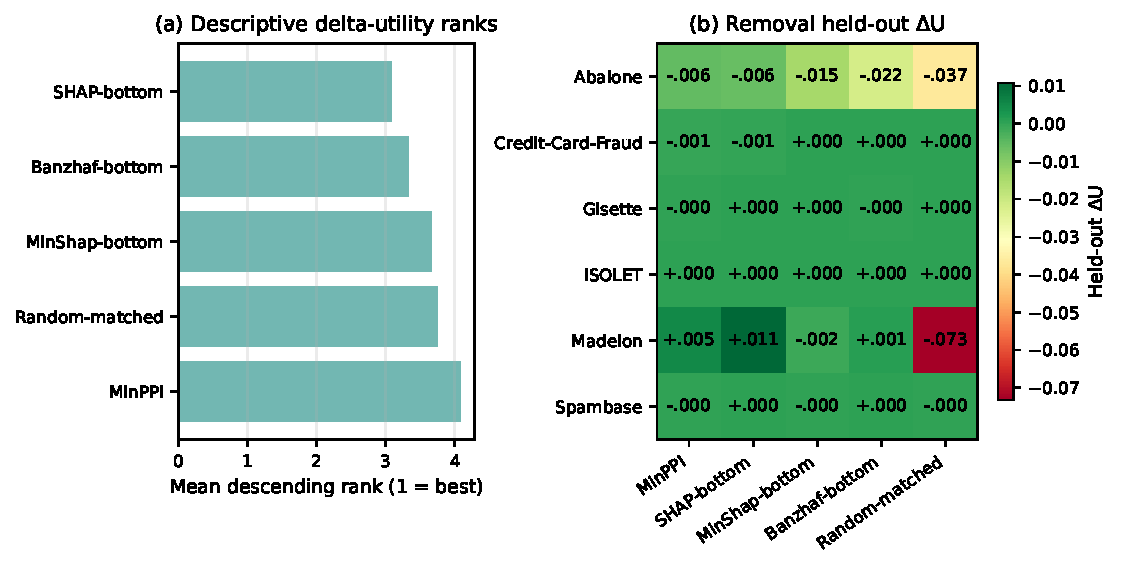
\includegraphics[width=\linewidth]{../figures/fig2_cd_heatmap.pdf}
\caption{Validation-gated matched removal. (a) Mean descending ranks (1 is best) of the six methods from their five-seed mean $\Delta U$ (full participates but is omitted). (b) Five-seed mean $\Delta U$; positive favors removal. Controls delete the accepted MinPPI-matched count, with 30 random-matched trials averaged per seed. Descriptive; no broad ordering claimed.}
\label{fig:removal}
\end{figure}

\section{Results}
\label{sec:results}

\subsection{RQ1: Validation-Gated Removal}



Table~\ref{tab:removal} shows heterogeneous compression: averaged over the 30 dataset--seed units, MinPPI removed 12.53\% of analyzed features with mean held-out $\Delta U=-.000313$ (nonzero removal in 14 of 30 units). Madelon had the largest compression (43.6\%) with $\Delta U=+.00469$, Abalone compressed by 27.5\% with $\Delta U=-.00565$, and Credit-Card-Fraud by \CreditCompression{} with $\Delta U=\CreditDeltaUtility{} $; the descriptive random-matched comparisons were $+.0047$ versus $-.0732$ on Madelon and $-.0056$ versus $-.0370$ on Abalone. The raw harmful set passed the validation gate in 27 of 30 units: 13 units had no candidates, and 14 of the 17 nonempty candidate sets passed. The three failed cases backed off to zero removal.



\begin{table}[htbp]
\caption{MinPPI removal at $\alpha=.95$ over five seeds. Compression and held-out $\Delta U$ are mean $\pm$ SD; ``raw pass'' counts validation-gate passes before backoff.}
\label{tab:removal}
\centering
\footnotesize
\begin{tabular}{lrrc}
\toprule
Dataset & Compression (\%) & Held-out $\Delta U$ & Raw pass \\
\midrule
Abalone & $27.50\pm25.62$ & $-.00565\pm.01077$ & $3/5$ \\
Credit-Card-Fraud & $2.76\pm2.89$ & $-.00078\pm.00335$ & $5/5$ \\
Gisette & $.60\pm.89$ & $-.00011\pm.00016$ & $5/5$ \\
ISOLET & $.00\pm.00$ & $.00000\pm.00000$ & $5/5$ \\
Madelon & $43.60\pm31.96$ & $+.00469\pm.00497$ & $4/5$ \\
Spambase & $.72\pm.99$ & $-.00003\pm.00007$ & $5/5$ \\
\bottomrule
\end{tabular}
\end{table}

\begin{table}[H]
\caption{Five-seed mean held-out utility after each variant deletes the accepted MinPPI-matched count; utility is AUC/OVR-AUC/$R^2$ by task, higher is better. SHAP/MinShap/Banzhaf/Random/Credit abbreviate SHAP-bottom/MinShap-bottom/Banzhaf-bottom/random-matched/Credit-Card-Fraud.}
\label{tab:utility}
\centering
\footnotesize
\begin{tabular}{lrrrrrr}
\toprule
Dataset & Full & MinPPI & SHAP & MinShap & Banzhaf & Random \\
\midrule
Madelon & .7876 & .7923 & .7985 & .7861 & .7884 & .7144 \\
Abalone & .5397 & .5340 & .5333 & .5251 & .5174 & .5027 \\
Credit & .9734 & .9726 & .9728 & .9736 & .9736 & .9736 \\
Gisette & .9887 & .9886 & .9887 & .9889 & .9887 & .9887 \\
ISOLET & .9935 & .9935 & .9935 & .9935 & .9935 & .9935 \\
Spambase & .9858 & .9858 & .9858 & .9856 & .9859 & .9858 \\
\bottomrule
\end{tabular}
\end{table}

Table~\ref{tab:utility} lists the held-out utilities achieved by the removal variants as a baseline comparison on the same deletion budget.

MinPPI's average utility across datasets was descriptively close to the full model (difference $-0.0003$, Wilcoxon $p = 0.44$), without establishing equivalence. Its mean rank among all methods was 4.08; the Friedman test gave $p = 0.89$, every MinPPI pairwise Wilcoxon comparison had raw $p \geq 0.4375$, and all corresponding Holm-adjusted values were $1.0$.
However, these mixed-scale averages are only descriptive. 
Together, these results indicate small average differences in this campaign, but they do not establish non-inferiority, equivalence, or significant improvement.
Figure~\ref{fig:removal} therefore visualizes heterogeneity rather than superiority.

Dataset heterogeneity was substantial. Madelon showed $43.6\%$ mean compression and held-out $\Delta U=+0.00469$, whereas Abalone showed $27.5\%$ compression and $\Delta U=-0.00565$. Credit-Card-Fraud, Gisette, and Spambase showed small average removal and small held-out changes, while ISOLET had zero accepted removal under the registered setting. These outcomes are descriptive and do not establish why a dataset did or did not admit accepted removals. The validation gate vetoed the raw harmful set in the two Abalone seeds and one Madelon seed that failed the validation loss bound, but it is not a held-out guarantee. Compression is seed-sensitive (SDs of $25$--$32$ percentage points on Madelon and Abalone), so the harmful set should be read as a five-seed aggregate.

\FloatBarrier
\subsection{RQ2: Quota Sensitivity}

\begin{figure}[H]
\centering
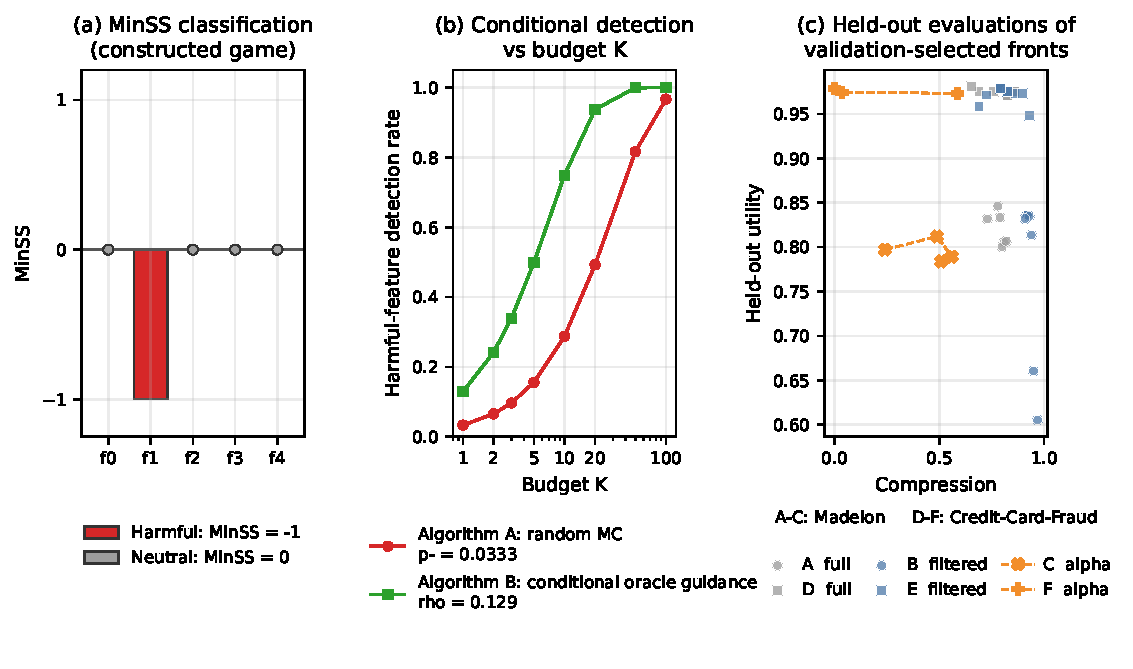
\includegraphics[width=\linewidth]{../figures/fig1_overview.pdf}
\caption{Overview of MinPPI. (a) Exact minimum marginals in the constructed game~\eqref{eq:constructed-game}: $f_1=-1$, the rest neutral. (b) Detection probability vs budget for random MC ($p_-=1/30=.0333$) and Algorithm B on the oracle seed $\{f_0,f_2\}$ ($\rho=.129$); illustrative, not real-data guidance evidence. (c) Seed-42 held-out fronts of full vs prefiltered NSGA-II with the registered $\alpha$ points on Madelon and Credit-Card-Fraud; connecting lines only order $\alpha$.}
\label{fig:overview}
\end{figure}

The $\alpha$ sweep is a seed-42 sensitivity analysis ($n=1$ per point), not a model-selection exercise. Its trajectories were dataset-dependent and non-monotone. On Madelon, compression across $\alpha=(.85,.90,.95,.99)$ was $(.24,.49,.56,.51)$ with held-out $\Delta U=(+.0077,+.0227,-.0003,-.0054)$. On Abalone, compression was $(.375,.50,.50,0)$, while on Credit-Card-Fraud it rose from 0 at $.85$ and $.90$ to $.034$ at $.95$ and $.586$ at $.99$. Figure~\ref{fig:overview}(c) overlays the registered points for Madelon and Credit-Card-Fraud on held-out evaluations of their seed-42 validation-selected fronts; the complete six-dataset sweep is reported in Table~\ref{tab:alpha} in the appendix. The points illustrate quota sensitivity only; they do not prove monotonicity, held-out nondominance, or cross-seed safety.

\FloatBarrier
\subsection{RQ3: Prefiltered Multi-Objective Search}

With the same 800-evaluation budget, MinPPI-prefiltered NSGA-II changed the dataset-averaged held-out hypervolume by $+.01584$ and validation hypervolume by $+.01741$. For each endpoint, all five seed-level pooled differences were positive (rank-biserial correlation 1), but the exact sign-flip $p=.0625$ became $.4375$ after the registered Holm correction. Dataset mean test-HV differences were $+.09515$ on Madelon, $+.00535$ on Credit-Card-Fraud, $+.00021$ on Abalone, 0 on ISOLET, $-.00191$ on Gisette, and $-.00378$ on Spambase. Thus the positive pooled direction is driven mainly by Madelon, with only small positive differences on Credit-Card-Fraud and Abalone.

On average, the post-hoc diagnostic reached 95\% of the final HV 22.67 evaluations earlier under MinPPI prefiltering, with the largest reductions on Madelon and Gisette and a slight increase on Spambase.  
Both variants nevertheless consumed the same registered total budget of 800 evaluations. Figure~\ref{fig:prefilter} therefore supports a directional, dataset-dependent change in search outcomes, not universal improvement, budget reduction, or runtime acceleration.

\begin{figure}[H]
\centering
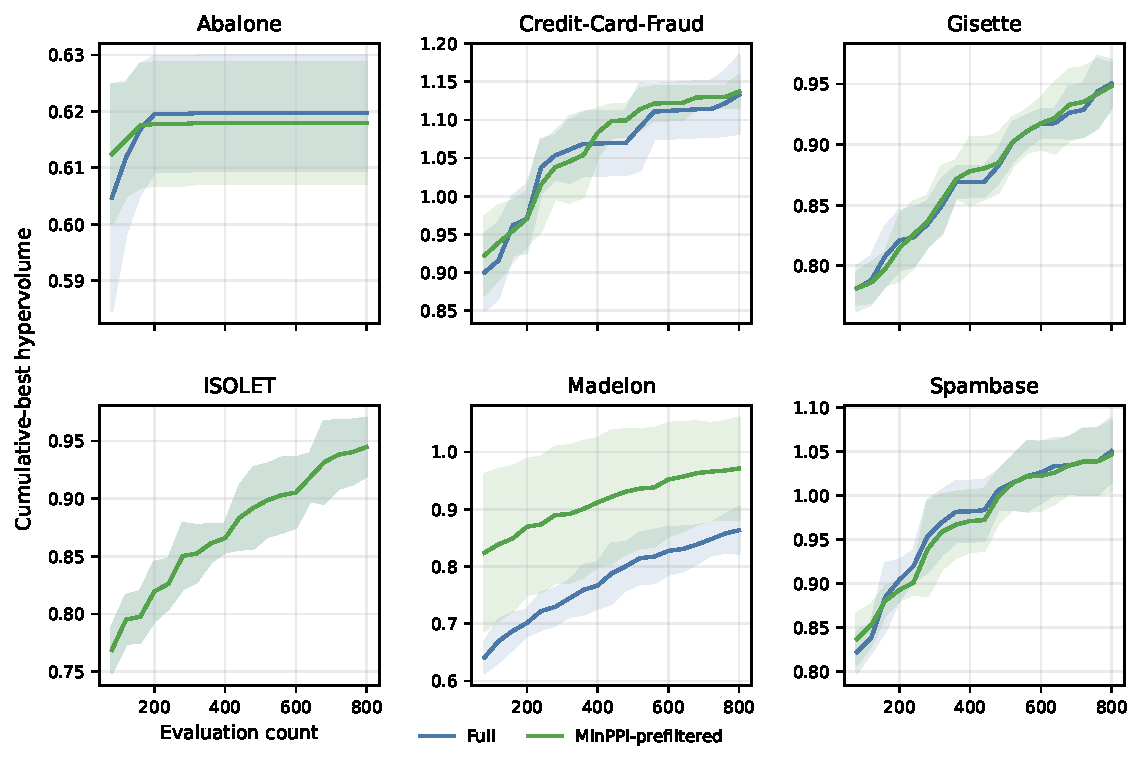
\includegraphics[width=\linewidth]{../figures/fig3_prefilter.pdf}
\caption{Hypervolume convergence of full vs MinPPI-prefiltered NSGA-II under the matched 800-evaluation budget. Each panel is a dataset; blue/green lines are five-seed means of cumulative-best validation hypervolume with $\pm$1-SD shading and reference point $(1.1,1.1)$. Curves coincide on most datasets and separate on Madelon; the dataset-averaged held-out change is \NsgaMeanHvChange{}. No dataset-wise comparison survives the registered Holm-corrected sign-flip tests.}
\label{fig:prefilter}
\end{figure}

\FloatBarrier
\subsection{RQ4: Estimator, Guidance, and Utility Sensitivity}

Abalone is the only dataset small enough for exact enumeration. Averaged over the five seed-level F1 scores, at budgets $2,5,10,25$, random MC achieved $.100,.150,.230,.443$, while MI-correlation guidance achieved $.000,.080,.133,.313$. The hybrid dispatcher scored 1 at every budget because it selected exact enumeration at eight features; this does not validate the approximate guidance heuristic. Thus the five-seed mean F1 for learned guidance was lower than random sampling at every registered finite budget; this is not a claim about every individual seed.

The ablations likewise show sensitivity rather than a stable guidance ordering. On Madelon, random, MI-only, correlation-only, and MI-correlation seeds recovered 5, 16, 34, and 28 harmful labels; on Credit-Card-Fraud the counts were 6, 2, 2, and 1. On ISOLET, changing the utility while keeping the probability-producing classifier fixed changed the harmful count from 0 under the formal OVR AUC to 9 under accuracy. These single-seed results show that estimator and utility choices materially affect recovered labels, but they cannot support significance or cross-seed stability claims.

A practical reading follows. Exact enumeration and the hybrid dispatcher recover every harmful label on Abalone, so MinPPI's reliable value lies in the exact or hybrid path when the dimension is small enough; the MI-correlation guidance is best treated as a fallback for larger problems, where it is not validated to improve on random sampling. The sensitivity of the recovered harmful set to estimator, seed construction, and utility likewise reinforces that MinPPI should be consumed as a conservative, validation-gated, multi-seed aggregate rather than a single configuration.



\FloatBarrier

\section{Discussion}
\label{sec:discussion}

The exact contribution of MinPPI is sharper than its empirical claim: an exact or sampled $-1$ is existence-certified by an evaluated threshold-crossing coalition, the validation gate separates witness discovery from removal, and finite sampling preserves witness validity but not completeness (a sampled 0 or $+1$ does not certify the exact class). MinPPI is a worst-case support statistic rather than an interaction index~\citep{grabisch1999axiomatic,rabitti2019shapley}, certifying a single harmful witness per feature rather than quantifying pairwise interactions. This matters because the study does not support a universal selector ranking: MinPPI stayed close to full-model utility yet had mean rank 4.08, and Abalone exhibited a negative held-out effect.

The downstream results are similarly conditional: Madelon drives most of the positive average hypervolume change, Credit-Card-Fraud and Abalone show small positive differences, and Gisette and Spambase small decreases. Prefiltering is useful when its accepted set removes distracting dimensions, but the study identifies no general dataset condition and establishes no statistical superiority, and the validation gate cannot guarantee held-out non-inferiority (it uses no test information by design).

These findings delimit where MinPPI may be useful. Under the registered setting it removes only candidates with evaluated harmful witnesses and only when a fixed validation-loss gate accepts the full candidate set. Its strongest descriptive result occurred on Madelon, while several datasets yielded little or no accepted removal and Abalone showed a held-out cost. Plausible applications are (i) prefiltering high-dimensional feature spaces before modeling or multi-objective search, (ii) auditing feature quality to flag suspicious or noisy predictors, and (iii) a validation-gated removal step for single-task models. These applications remain hypotheses for broader replication; the output here should be read as a five-seed aggregate conditional on the frozen model, split, utility, quota, estimator, and gate.

Several limitations constrain interpretation. First, five paired seeds and six datasets give low-powered tests, and the ablations use only seed 42. Second, a single XGBoost family and mixed utility scales make a common multiplicative quota non-invariant to utility shifts. Third, exact estimator comparison is available only on eight-feature Abalone, where guidance F1 was below random sampling at every budget; the detection bound~\eqref{eq:detection} is a support condition, not evidence that guidance assigns more mass to harmful witnesses. Fourth, shared caching complicates runtime attribution, so we make no speedup claim. Finally, paired seed-level variation, broader model families, a stronger learned-guidance estimator, standard filter/wrapper baselines, and extending harmful-feature removal to multi-task settings remain future work.

\section{Conclusion}

Exact MinPPI specializes minimum marginal aggregation to a binary utility-threshold game and yields a quota-conditioned three-way classification; finite-budget estimators certify only observed harmful threshold crossings. The resulting candidates feed a validation-gated removal or prefiltering step. Across the six benchmark datasets, mean compression was 12.5\% with mean held-out $\Delta U=-0.00031$; Madelon provided the clearest descriptive removal result, and the average hypervolume change in prefiltered search was positive but non-significant after correction. Removal superiority, a general guidance advantage, runtime reduction, and held-out non-inferiority were not established. The appropriate conclusion is therefore methodological and conditional: MinPPI provides witness-certified semantics for observed harmful features, while the value of acting on those witnesses depends on the model, split, dataset, estimator, utility, quota, and validation decision---consistent with the observation that harmful features are context-dependent rather than universally removable~\citep{lippl2024inductive}.

\bibliography{icomp2026_conference}
\bibliographystyle{icomp2026_conference}

\appendix

\section{Proofs}
\label{app:proofs}

\begin{proof}[Proof of Proposition~1]
Because $v_\alpha\in\{0,1\}$, every marginal $\Delta_i(S)$ is in $\{-1,0,+1\}$, and so is any nonempty minimum of such marginals. For each $S\subseteq N\setminus\{i\}$ there are $|S|!(n-|S|-1)!\geq1$ permutations for which $S$ is exactly the predecessor set of $i$. Hence the distinct arguments of $\operatorname{MinSS}_i$ and $\operatorname{MinBz}_i$ coincide; multiplicity cannot change a minimum.

The minimum equals $-1$ if and only if at least one marginal is $-1$, which is equivalent to the existence of $S$ with $v_\alpha(S)=1$ and $v_\alpha(S\cup\{i\})=0$. It equals $+1$ if and only if every marginal is $+1$, which is equivalent to $v_\alpha(S)=0$ and $v_\alpha(S\cup\{i\})=1$ for every $S$. If neither condition holds, the trinary range forces the minimum to be 0.
\end{proof}

\begin{proof}[Finite-sample one-sidedness]
For any sampled collection $\mathcal{S}_K\subseteq2^{N\setminus\{i\}}$,
\[
\min_{S\in\mathcal{S}_K}\Delta_i(S)
\geq
\min_{S\subseteq N\setminus\{i\}}\Delta_i(S),
\]
because the left minimum is taken over a subset of the right minimum's arguments. An observed value $-1$ is therefore exact evidence of at least one harmful witness, but a larger sampled minimum can result from an unseen smaller marginal.
\end{proof}

\begin{proof}[Conditional detection bound]
Let independent perturbations be drawn from $P_i$, and suppose a fixed harmful witness $S_i^*$ has mass $\rho_i>0$. One draw misses that witness with probability $1-\rho_i$; all $K_{\mathrm{adv}}$ draws miss it with probability $(1-\rho_i)^{K_{\mathrm{adv}}}$. Sampling $S_i^*$ implies detection, which yields~\eqref{eq:detection}. The statement is silent when $\rho_i=0$ and does not compare $P_i$ with the random-MC distribution.
\end{proof}

\section{Quota Sweep}

Table~\ref{tab:alpha} reports the seed-42 $\alpha$ sweep (compression, held-out $\Delta U$) for the six benchmark datasets; the non-monotone rows complement the RQ2 discussion.

\begin{table}[H]
\caption{Quota operating points, shown as (compression, held-out $\Delta U$). Every cell has $n=1$.}
\label{tab:alpha}
\centering
\scriptsize
\begin{tabular}{lcccc}
\toprule
Dataset & $\alpha=.85$ & $\alpha=.90$ & $\alpha=.95$ & $\alpha=.99$ \\
\midrule
Abalone & $(.375,+.0041)$ & $(.500,-.0198)$ & $(.500,+.0010)$ & $(0,0)$ \\
Credit-Card-Fraud & $(0,0)$ & $(0,0)$ & $(.034,-.0045)$ & $(.586,-.0057)$ \\
Gisette & $(0,0)$ & $(0,0)$ & $(0,0)$ & $(.090,+.0002)$ \\
ISOLET & $(0,0)$ & $(0,0)$ & $(0,0)$ & $(.010,-.000005)$ \\
Madelon & $(.240,+.0077)$ & $(.490,+.0227)$ & $(.560,-.0003)$ & $(.510,-.0054)$ \\
Spambase & $(0,0)$ & $(0,0)$ & $(0,0)$ & $(.196,-.0012)$ \\
\bottomrule
\end{tabular}
\end{table}

\section{Reproducibility Details}

The formal splits are 64\%/16\%/20\% train/validation/test; dataset identities, split indices, transformations, model policy, source, and scientific environment are recorded with cryptographic digests, and resume rejects protocol drift. Training data fit preprocessing, guidance, and all coalition models; validation is reused adaptively for threshold-game construction, the removal gate, and NSGA-II selection, while the held-out partition is read only for registered evaluation. The original seven-dataset campaign is retained as the historical record; a post-hoc integrity audit excluded Communities \& Crime from the publication analysis for outcome-component leakage, and the reported tables and figures were recomputed for the six retained datasets. The estimator set, removal controls, and NSGA-II variants are as in Section~3; runtime counters are diagnostic only. Tables and figures are rederived from canonical row-level records and independently hash-verified.

\end{document}
